%%%% ijcai11.tex

%TODO: hoogte onderaan kleiner maken
%TODO: use short names for frameworks throughout the paper
%TODO: welke afkorting nu voor Kendo UI? KUI of Kendo? Sander: Kendo
%TODO: welke afkorting in de captions van tabellen/figuren?

\typeout{IJCAI-11 Instructions for Authors}

% These are the instructions for authors for IJCAI-11.
% They are the same as the ones for IJCAI-07 with superficical wording
%   changes only.

\documentclass[a4paper]{artikel3}
% The file ijcai11.sty is the style file for IJCAI-11 (same as ijcai07.sty).
\usepackage{ijcai11}

% Use the postscript times font!
\usepackage{times}


% the following package is optional:
%\usepackage{latexsym} 

%%%%%%%%%%%%%% CUSTOM BEGIN %%%%%%%%%%%%%%

% remove if not a draft
\usepackage{draftwatermark}
\SetWatermarkColor[rgb]{0.90,0.90,0.90}

\usepackage[english]{babel}
\usepackage[utf8]{inputenc}
\usepackage[colorlinks]{hyperref}
\usepackage{multirow}
\usepackage{pgfplotstable} %nodig voor CSV to Latex
\usepackage{booktabs} % voor layout comparisontable
\usepackage{amsmath}

%\usepackage[hyphens]{url}


% captions
\usepackage{caption} 
\captionsetup{margin=10pt,font=small,labelfont=bf}

% engelse term die we niet vertalen naar het nederlands
\newcommand{\term}[1]{\emph{#1}}

% code commande
\newcommand{\code}[1]{\texttt{#1}}

% zodat we niet http:// staan hebben in onze tekst, maar de link wel werkt
\newcommand{\exturl}[1]{\href{http://#1}{#1}}
\renewcommand{\url}[1]{\href{#1}{#1}}


% paragraphs anders te feel white space
\usepackage{setspace}
\newcommand{\setspace}[0]{\vspace{2mm}}
\renewcommand{\paragraph}[1]{\setspace \noindent {\bf #1}  }
\newcommand{\framework}[2]{ \emph{#1 (\textbf{#2}): }} %enkel in usage stukje om framework in te leiden

\newcommand{\challenge}[1]{\paragraph{#1}}

\newcommand{\jqm}[0]{jQuery Mobile}
\newcommand{\jqma}[0]{jQM}
\newcommand{\st}[0]{Sencha Touch}
\newcommand{\sta}[0]{ST}
\newcommand{\kendo}[0]{Kendo UI}
\newcommand{\kendoa}[0]{Kendo}
\newcommand{\lungo}[0]{Lungo}
\newcommand{\lungoa}[0]{Lungo}
\newcommand{\tmp}[0]{The-M-Project}
\newcommand{\quo}[0]{QuoJS}
\newcommand{\moobile}[0]{Moobile}
\newcommand{\davinci}[0]{DaVinci}
\newcommand{\jqt}[0]{jQT}
\newcommand{\js}[0]{JavaScript}
\newcommand{\htc}[0]{HTCDesireZ}
\newcommand{\gtab}[0]{GalaxyTab}
\newcommand{\gs}[0]{GalaxyS}
\newcommand{\nexus}[0]{Nexus 7}
\newcommand{\ipadi}[0]{iPad1 WiFi}
\newcommand{\ipadiii}[0]{iPad3 4G WiFi}
\newcommand{\iphoneiii}[0]{iPhone 3GS}
\newcommand{\iphoneiv}[0]{iPhone 4S}
\usepackage{pdftexcmds}
\makeatletter
\newcommand{\uit}[1]{
	\ifnum\pdf@strcmp{#1}{anatomie}=0
  		U1:~Anatomie van pagina%
	\else\ifnum\pdf@strcmp{#1}{toestel}=0
    	U2:~Toestelspecifieke lay-out%
	\else\ifnum\pdf@strcmp{#1}{laadscherm}=0
    	U3:~Laadscherm en dialoogvenster%
	\else\ifnum\pdf@strcmp{#1}{formulieren}=0
    	U4:~Formulieren%
	\else\ifnum\pdf@strcmp{#1}{formulieren-placeholders}=0
    	U4.1:~Maak formulieren met placeholders zonder labels%
	\else\ifnum\pdf@strcmp{#1}{formulieren-types}=0
    	U4.2:~Gebruik tekst/nummer/e-mail als formuliertypes%
  	\else\ifnum\pdf@strcmp{#1}{formulieren-optieveld}=0
    	U4.3:~Optieveld%
  	\else\ifnum\pdf@strcmp{#1}{formulieren-datepicker}=0
    	U4.4:~Aangepaste datepicker met bereik van data%
  	\else\ifnum\pdf@strcmp{#1}{formulieren-monthpicker}=0
		U4.5:~Aangepaste datepicker met enkel maand- en jaarveld%
  	\else\ifnum\pdf@strcmp{#1}{formulieren-schakelaar}=0
		U4.6:~Schakelaar%
  	\else\ifnum\pdf@strcmp{#1}{formulieren-wissen}=0
		U4.7:~Wissen van een formulier%
	\else\ifnum\pdf@strcmp{#1}{vullen}=0
    	U5:~Automatisch invullen van formulier%
	\else\ifnum\pdf@strcmp{#1}{autoaanvullen}=0
    	U6:~Auto-aanvullen%
	\else\ifnum\pdf@strcmp{#1}{afbeelding}=0
    	U7:~Toevoegen van afbeelding%
	\else\ifnum\pdf@strcmp{#1}{validatie}=0
    	U8:~Formuliervalidatie%
	\else\ifnum\pdf@strcmp{#1}{handtekening}=0
    	U9:~Handtekening%
	\else\ifnum\pdf@strcmp{#1}{ajax}=0
    	U10:~AJAX%
	\else\ifnum\pdf@strcmp{#1}{lijsten}=0
    	U11:~Lijsten%
	\else\ifnum\pdf@strcmp{#1}{pdf}=0
    	U12:~Toon PDF%
	\else\ifnum\pdf@strcmp{#1}{offline}=0
  		U13:~Offline%
	\else\ifnum\pdf@strcmp{#1}{offline-data}=0
  		U13.1:~Bewaar data%
	\else\ifnum\pdf@strcmp{#1}{offline-app}=0
		U10.3:~Maak de applicatie offline beschikbaar%
  	\else
		[?]%
		
  	\fi\fi\fi\fi\fi
  	\fi\fi\fi\fi\fi
  	\fi\fi\fi\fi\fi
  	\fi\fi\fi\fi\fi
  	\fi\fi
}

\newcommand{\chal}[2]{
	\ifnum\pdf@strcmp{#1}{anatomie}=0
		C1:~Anatomy of page%
	\else\ifnum\pdf@strcmp{#1}{toestel}=0
		C2:~Device-specific layout%
  	\else\ifnum\pdf@strcmp{#1}{laadscherm}=0
		C3:~Load screen and dialog%
	\else\ifnum\pdf@strcmp{#1}{formulieren}=0
		C4:~Forms%
  	\else\ifnum\pdf@strcmp{#1}{formulieren-placeholders}=0
    	C4.1:~Create forms with placeholders without labels%
  	\else\ifnum\pdf@strcmp{#1}{formulieren-types}=0
    	C4.2:~Use the text/number/email as form types%
  	\else\ifnum\pdf@strcmp{#1}{formulieren-optieveld}=0
   	 	C4.3:~Option field%
  	\else\ifnum\pdf@strcmp{#1}{formulieren-datepicker}=0
    	C4.4:~Custom datepicker with data range%
  	\else\ifnum\pdf@strcmp{#1}{formulieren-monthpicker}=0
		C4.5:~Custom datepicker only with month and year%
  	\else\ifnum\pdf@strcmp{#1}{formulieren-schakelaar}=0
		C4.6:~Flip switch%
  	\else\ifnum\pdf@strcmp{#1}{formulieren-wissen}=0
		C4.7:~Clearing the form%
  	\else\ifnum\pdf@strcmp{#1}{vullen}=0
		C5:~Automatic form filling%
	\else\ifnum\pdf@strcmp{#1}{autoaanvullen}=0
		C6:~Autocomplete%
	\else\ifnum\pdf@strcmp{#1}{afbeelding}=0
		C7:~Attach image%
	\else\ifnum\pdf@strcmp{#1}{validatie}=0
		C8:~From validation%
	\else\ifnum\pdf@strcmp{#1}{handtekening}=0
		C9:~Signature%
	\else\ifnum\pdf@strcmp{#1}{ajax}=0
		C10:~AJAX%
  	\else\ifnum\pdf@strcmp{#1}{lijsten}=0
		C11:~Lists%
  	\else\ifnum\pdf@strcmp{#1}{pdf}=0
		C12:~Show PDF%
  	\else\ifnum\pdf@strcmp{#1}{offline}=0
		C13:~Offline%
  	\else\ifnum\pdf@strcmp{#1}{offline-data}=0
  		C13.1:~Saving data%
  	\else\ifnum\pdf@strcmp{#1}{offline-app}=0
  		C13.2:~Making app offline%
	\else
    	[?]%
	
  	\fi\fi\fi\fi\fi
  	\fi\fi\fi\fi\fi
  	\fi\fi\fi\fi\fi
  	\fi\fi\fi\fi\fi
  	\fi\fi
}
\makeatother

%%%%%%%%%%%%%% CUSTOM END %%%%%%%%%%%%%%

% Following comment is from ijcai97-submit.tex:
% The preparation of these files was supported by Schlumberger Palo Alto
% Research, AT\&T Bell Laboratories, and Morgan Kaufmann Publishers.
% Shirley Jowell, of Morgan Kaufmann Publishers, and Peter F.
% Patel-Schneider, of AT\&T Bell Laboratories collaborated on their
% preparation.

% These instructions can be modified and used in other conferences as long
% as credit to the authors and supporting agencies is retained, this notice
% is not changed, and further modification or reuse is not restricted.
% Neither Shirley Jowell nor Peter F. Patel-Schneider can be listed as
% contacts for providing assistance without their prior permission.

% To use for other conferences, change references to files and the
% conference appropriate and use other authors, contacts, publishers, and
% organizations.
% Also change the deadline and address for returning papers and the length and
% page charge instructions.
% Put where the files are available in the appropriate places.

%TODO toevoegen header dingen van gonzalo
\title{Comparative study of frameworks for \\ the development of mobile HTML5 applications}
\author{Tim Ameye \\ tim.ameye@student.kuleuven.be \And Sander Van Loock \\ sander.vanloock1@student.kuleuven.be}
\begin{document}

\maketitle

\begin{abstract}
The need to make mobile applications that run on every device is ever-growing.
One solution is to build mobile web applications using HTML5.
To speed up development, different frameworks exist that help in functionality and building a user interface.
Because of the variety of existing frameworks, a thorough comparative study is needed to know which framework suits the job best.
This paper compares \st{}, \jqm{}, \kendo{} and \lungo{} by using popularity, productivity, usage, support and performance as comparison criteria. 
The conclusion is that \jqm{} is the best framework with great productivity and performance. 
\kendo{} gets the second place and its main asset is usage.
\lungo{} is third and has the fastest download performance.
\st{} ends last but gets the best user experience.
Furthermore all four frameworks have good support.
\end{abstract}

%%%%%%%%%%%%%%%%%%%%%%%%%%%%%%%%%%%%%%%%%%%%%%%%%%%%%%%%%%%%%%%%%%%%%%%%%%%%%%%%%%%%%%%
%%%%%%%%%%%%%%%%%%%%%%%%%%%%%%%%%%%%%%%%%%%%%%%%%%%%%%%%%%%%%%%%%%%%%%%%%%%%%%%%%%%%%%%

\section{Introduction} % (1 blz)
\label{sec:introduction}
Since the release of the Apple iPhone in 2007~\cite{David2011}, the demand for smartphones is ever since increasing. 
Today, over one billion smartphones are in use globally~\cite{Yang2012}.
This will double by 2015~\cite{Gillett2012}.
Also tablets conquer market share as mobile devices.
760 million tablets will be in use globally by 2016~\cite{Gillett2012}.
Besides Apple, other companies like Google and Microsoft are on the track too.
All those mobile devices come in different shapes and sizes.
They also include different features like GPS, camera and connectivity like Bluetooth, WiFi and 3G.

On these mobile devices run mobile operating systems~(OS). The two mobile OSs with the greatest market share are iOS and Android with 14.9\% and 75.0\% respectively in Q3 of 2012~\cite{Protalinski2012}.
These mobile OSs run both on smartphones and tablets.

The mobile OS from Apple, called iOS, first appeared in 2007.
Since then, a new version was released every year with the most recent version being iOS~6.1 which was released in January~2013~\cite{Deitel2012,PhilDutson2012,Apple2013}.
The mobile browser from Apple shipped with iOS is called Mobile Safari.
Apple did make sure to catch up with the latest HTML5 specifications in its browser~\cite{Hales2012}.
This was also because of the dropped support for Adobe Flash on their mobile devices~\cite{Jobs2010}.

In 2005, Google bought Android Inc. and released its first stable mobile OS, called Android, in 2008~\cite{Satyesh2012}.
Like with iOS, new versions were released on a yearly basis.
Android~4.2 is the latest version and was released in October 2012~\cite{Sawers2012}.
Android comes with the Android browser.
The implementation of HTML5 specifications has dragged, but as of Android 4.0, support is increasing~\cite{Hales2012}.
It is now also possible to install the mobile version of the Chrome desktop browser on devices with Android 4.0 and later.

It is important to look at the usage of the different OS versions, which is shown in table~\ref{table:mos-versions}.
This is because not every user has (updated to) the latest version on his mobile device.
The table shows that almost 90\% of iOS users already has version iOS~6.x.
In contrast, about a half of the Android users is still using Android~2.x while the latest major version is Android~4.x. 
Those users cannot benefit of the latest bells and whistles, particularly the new features of HMTL5, on their devices.

\begin{table}[t]
\centering
\pgfplotstabletypeset[
  begin table=\begin{tabular}{l l},
  end table=\end{tabular},
  col sep=comma,
  header=true,
  string type,
  skip coltypes=true,
  columns={Versie,Marktaandeel},
  columns/Versie/.style={column name=\textbf{iOS}},  
  columns/Marktaandeel/.style={column name=\textbf{Share (\%)}},
  every head row/.style={
    before row=\toprule,
    after row=\midrule},
  every last row/.style={
    after row=\bottomrule}
]{../Masterproef/tabellen/ios.csv}
\quad
\pgfplotstabletypeset[
  begin table=\begin{tabular}{l l},
  end table=\end{tabular},
  col sep=comma,
  header=true,
  string type,
  skip coltypes=true,
  columns={Versie,Marktaandeel},
  columns/Versie/.style={column name=\textbf{Android}},  
  columns/Marktaandeel/.style={column name=\textbf{Share (\%)}},
  every head row/.style={
    before row=\toprule,
    after row=\midrule},
  every last row/.style={
    after row=\bottomrule}
]{../Masterproef/tabellen/android.csv}
\caption{Usage of iOS versions on May 8, 2013 and Android versions on May 1, 2013 \protect\cite{Smith2013,Android2013}.}
\label{table:mos-versions}
\end{table}

There are three possible ways to make a mobile application~\cite{Accenture2012,Hales2012}.
The first one is a \emph{web application} which runs entirely in the browser.
The second type of application is a \emph{native application} which is installed on the device and programmed in a language specific to the mobile OS.
Lastly, a mix of both can be made which is called a \emph{hybrid application}.
One approach is to pack the web application as a native application.
The other approach is to use one programming language to build native applications for different OSs.

Advantages of web applications are the presence of a browser on mobile devices, so everyone can use it directly without installing the app first and regardless of their mobile OS~\cite{Accenture2012}.
Secondly, the code needs only to be written once and can be run anywhere (WORA)~\cite{Hales2012}.
This is in contrast to native, were a codebase has to be maintained for every mobile OS.
Lastly, web applications do not need to be published to a store (e.g. App Store for iOS and Google Play for Android) prior to release.
Such a store is a place where users can download application to their mobile device.
A disadvantage of web applications is that they are dependent on the mobile OS just like native applications.
This is especially the case when using new features of HTML5 in web applications.

In contrast, native applications provide better performance~\cite{Accenture2012}.
Secondly, it is easier to use features like GPS and camera of the mobile device with a native application.
Thirdly is a security issue were web applications lack behind.
Lastly, publishing applications through a store has two advantages.
On the one hand it increases publicity.
On the other hand stores can also control the quality of the applications, which is not the case for web applications.

The advantage of hybrid applications is that they patch the issues of web applications with the benefits of native applications.
However, as of December 2012, HTML5 went into candidate recommendation~\cite{Jacobs2012}.
This implies the upcoming support of HTML5 in contemporary browsers and that hybrid applications will probably become obsolete over time.

%%%%%%%%%%%%%%%%%%%%%%%%%%%%%%%%%%%%%%%%%%%%%%%%%%%%%%%%%%%%%%%%%%%%%%%%%%%%%%%%%%%%%%%
%%%%%%%%%%%%%%%%%%%%%%%%%%%%%%%%%%%%%%%%%%%%%%%%%%%%%%%%%%%%%%%%%%%%%%%%%%%%%%%%%%%%%%%

\section{Related Work} % Sander 0.25 pg
\label{sec:related-work}

%TODO related work buiten HTML5, native? anders literatuur buiten vergelijkingscriteria?

In the literature, many frameworks are presented, but not compared.
If they do get compared, none of them are scientifically published or use a proof of concept (POC) to validate their comparison.  
The idea of using a POC is not new.  
Oehlman~\cite{Oeflman2011} and Kosmaczewski~\cite{Kosmaczewski2012},  for example,  use a small geosocial game and todo list application respectively to present mobile HTML5 frameworks.

Some blog posts \cite{Sarrafi2012a,Ayuso2012,Rozynski2011} all have their own criteria and methodologies to assess different mobile frameworks.  
The overall application of the criteria changes from use case to use case.  
Rozynski~\cite{Rozynski2011} presents the chosen criteria and discusses them for each framework.  
Ayuso~\cite{Ayuso2012} presents 17 criteria but all of them are discussed at once per framework.  
Thereafter,  advantages and disadvantages are subtracted and proposed to the reader.  
Finally, Sarrafi~\cite{Sarrafi2012a} presents their chosen criteria together with a scorecard and an explanation of scores per criterion.  
Each framework gets evaluated based on the scores for each criterion.

All these blog posts compare mobile and hybrid frameworks.  
Some websites~\cite{Bristowe2012,Burris} only focus on two mobile HTML5 frameworks in contrast to the Mobile Frameworks Comparison Chart from from Falk~\cite{Falk2011} that tries to compare as much as frameworks as possible in a large tabular form.

The report about Cross-Platform Developer Tools from Vision Mobile~\cite{Mobile2012} compares $15$ cross-platform tools.
One of these is Sencha.
The evaluation is based on a questionaire with more than 2400 deverlopers worldwide.
Their main focus lies on hybrid applications because they state that hybrid applications try to combine the best of both web and native applications.
This paper avoids this discussion and tries to find the best framework for building web applications.

The ISO 25010 standaard evaluates the productquality and quality in use of software~\cite{Standard2010}.
HTML5 frameworks could also be assessed with this standard.
The general methodology it uses is not applicable for HTML5 frameworks.
Security,  for example,  is not an issue for framework vendors.


%%%%%%%%%%%%%%%%%%%%%%%%%%%%%%%%%%%%%%%%%%%%%%%%%%%%%%%%%%%%%%%%%%%%%%%%%%%%%%%%%%%%%%%
%%%%%%%%%%%%%%%%%%%%%%%%%%%%%%%%%%%%%%%%%%%%%%%%%%%%%%%%%%%%%%%%%%%%%%%%%%%%%%%%%%%%%%%

\section{Comparison criteria} %Sander 0.75 pg
\label{sec:comparisoncriteria}

%TODO waarom criteria niet gekozen

The comparison study will be driven by a proof of concept (POC).  
This POC encompasses an application that allows employees to attach, sign and submit expenses to their employer.
Afterwards, the employee can view the uploaded expenses and download them as PDF.

Five important criteria will be used:  popularity,  productivity,  usage,  support and performance. 
The POC can be used in all but the first.   
A methodology that results in a score for each criterion will be described below.  
Per criterion,  a table or graph will be provided to give an overview of the total scores
At the final stage,  these scores will be plotted in a spider graph~\cite{Few2005}.   

\paragraph{Popularity}
%TODO Tim: oude tekst
%The activity around frameworks in social media has to be considered with a lot of care.  
%If,  for example,  a framework has a lot of questions on Stack Overflow,  one could conclude the framework has a lot of ambiguity.  
%Someone else could argue  the framework has a large active Internet community build around it.  
%Also,  the numbers of Twitter followers and Facebook likes only give an indication of the popularity of the framework,  there is no exact science involved.
Social networks provide a good indication to determine the popularity that goes with the framework.  
%\cite{Sarrafi2012a,Ayuso2012} use 
Twitter followers,  GitHub stars,  GitHub forkers,  Stack Overflow questions and Facebook likes will be recorded.
The summation of these five numbers give the score for the framework's popularity.  

% \begin{equation}
%   POP_f = T_f+S_f+F_f+SO_f+FB_f
%   \label{eq:populariteit}
% \end{equation}

\paragraph{Productivity}
Both autors implement the POC two different framework and carefully record the time to implement it.  
However,  this time will be influenced by many factors.
The second implementations will have an advantage because of the gained experience after the first implementation.
Also,  code reuse and possible incomplete implementations because of the limited functionality of the framework, affect this times in a negative way.
A better criterion will be the hours to partially implement the POC.  
The partial implementation contains the POC's login that loads a long list.
This application is not subjected to the influences described above. %TODO verder verklaren?
The time to implement the login application gives the score for the framework's productivity. 

% \begin{equation}
%   PROD_f = t_{f,login}
%   \label{eq:productiviteit}
% \end{equation}

\paragraph{Usage}
The POC will be subdivided in $13$ challenges and $38$ subchallenges.  
The score of this criterion will depend on the completion of the challenges by the framework.  
The assessment of the challenges can be found in table~\ref{table:challenges-scores}.  
The total of all challenges gives the score for the framework's usage.

\begin{table}[h]	
\centering
\begin{tabular}{ll}
\toprule
\textbf{Score} & \textbf{Assessment criteria}\\
\midrule
$C_{f,i} = 2$ & Supported by the framework\\
$C_{f,i} = 1$ & A plugin or HTML5 feature is needed\\
%TODO: beter woord vinden
$C_{f,i} = 0$ & No, custom or hacky implementation\\
\bottomrule
\end{tabular}
\caption{Assessment criteria for implementation challenges.}
\label{table:challenges-scores}
\end{table}

\begin{equation}
  \text{Usage}_f = \sum_{i=1}^{38}{\left(C_{f,i}\right)}
  \label{eq:gebruik}
\end{equation}

\paragraph{Support}
This criterion indicates the correct functionality of the POC implementation on different contexts.
A context is a combination of a particular operatingsystem, device and browser.
Both Android and iOS, smartphones and tablets will be checked.
Only native browsers will be looked at.
In total, eight contexts will be checked for support.
%,  similar as the cross-platform capabilities of~\cite{Sarrafi2012a}.  
In each context,  a subset of the challenges from the previous criterion will be checked.  
These are the challenge where the framework actually provided an implementation ($C_{r,i} > 0$).
If the challenge works as expected $C_{f,c,i} = 1$.
If some part of challenge is infeasible $C_{f,c,i} = 0$.
The summation of scores for each context will give the score for the framework's support.

\begin{equation}
  \text{Support}_f = \sum_{c=1}^{8}{\left(\sum_{i=1}^{N_f}C_{f,c,i}\right)}
  \label{eq:ondersteuning}
\end{equation}

\paragraph{Performance}
The download time of an HTML5-application is a major bottleneck for performance.
Therefor,  the loading time of the POC ($l_{f,c,POC}$) and login application ($l_{f,c,login}$) will be measured on eight devices.
Also,  the loading time for a cached version of both the POC ($l_{f,c,POC_{cache}}$) and login application ($l_{f,c,login_{cache}}$) will be recorded.
The summation of these loading times on $8$ devices, provide the average download time.

%TODO links uitlijnen
\begin{equation}
\begin{split}
\text{Average download time}_f =  \\ \frac{\sum_{c=1}^{8}\left(l_{f,c,POC}+l_{f,c,POC_{cache}}+ l_{f,c,login} + l_{f,c,login_{cache}}\right)}{8}
  \label{eq:dowloadtime}
\end{split}
\end{equation}

The responsetime of a list with $850$ elements will be measured on each context with two user tests ($\text{experience}_{f,c}$).
Calculating the responsetime with \js{} is not possible because \sta{} and \lungo{} do not have an event after the elements are rendered.
The result will be a total ordening of the frameworks per context that indicate the responsiveness.
The summation of the results will provide a factor to weight the average download time.
The formula for the framework's performance then becomes:

\begin{equation}
  \text{Performance}_f =  \frac{\text{Average download time}_f}{\sum_{c=1}^{8}{\text{experience}_{f,c}}}
  \label{eq:performance}
\end{equation}

%%%%%%%%%%%%%%%%%%%%%%%%%%%%%%%%%%%%%%%%%%%%%%%%%%%%%%%%%%%%%%%%%%%%%%%%%%%%%%%%%%%%%%%
%%%%%%%%%%%%%%%%%%%%%%%%%%%%%%%%%%%%%%%%%%%%%%%%%%%%%%%%%%%%%%%%%%%%%%%%%%%%%%%%%%%%%%%

\section{Frameworks} % (0.5 blz per framework + tabel)
\label{sec:frameworks}
This section introduces the compared mobile HTML5 frameworks: \st{}, \kendo{}, \jqm{} and \lungo{}.
%TODO: tekst over de 3 mogelijkheden om webapps te maken hier naar boven plaatsen?

\subsection{\st} % (0.5 blz Sander)
\label{sec:frameworks-sencha-touch}

\st{}~(\sta{}) is a framework developed by Sencha,  a company founded in 2010 as a composition of Ext JS, jQuery Touch and Raphaël.  
The first stable version of \sta{} was officialy released in November 2010.
Ext JS is a JavaScript framework for the development of HTML5 applications.  
jQuery Touch is a jQuery plugin for mobile development that adds touch events to jQuery and depends on the WebKit engine.  
Finally,  Raphaël, is a JavaScript library for vector drawings.  
Parts of the first two technologies can be found in the implementation of the \sta{} framework.    

As at the time of writing,  \sta{} is at version 2.2~\cite{Inc.}.

\paragraph{Documentation}
The documentations describes all object and features,  some with code examples and live previews~\cite{Inc.2013a}.
The key concepts of \sta{} are explained in tutorials:  some are texts, some are videos.  

A usefull tool to discover the \sta{} features is the Kitchen Sink~\cite{Inc.2013}.  
This is a HTML5-application that lines up all possibilities of the framework combined with the corresponding code.

\paragraph{License}
\sta{} is free within a commercial context in which the developer does not share the code with its users.  
There is also the option to use an open-source version.  
This comes with a GNU GPLv3 license which implies a free code redistribution as most important property.
Other licenses can be found at~\cite{SenchaInc.}.
  
\paragraph{Code and development}
\sta{} is written on top of Ext JS and can also be considered as a JavaScript framework.  
All code needs to be written in JavaScript and loaded by one HTML-container.  
Another important aspect of \sta{} is that it imposes the Model-View-Controller (MVC) architecture.  
Models group fields to data objects,  views define how the content is presented to the user and controllers connect both based on events.

\sta{} contains all UI elements as JavaScript objects.  
Just like object-oriented programming,  those objects are part of a class system.  
Classes can be defined and/or created.  
Single inheritance and overriding is also possible.    

To enhance performance,  it is the programmer's task to create components before they are used.  
In this way,  the programmer partially determines the performance of the application.

\paragraph{Browser support}
Just like jQuery Touch,  \sta{} is based upon the WebKit browser engine.  
This forms the major requirement for browser support.  
Although most mobile browsers contain this engine,  some like FireFox Mobile and Opera Mobile lack behind~\cite{JohnEClark2012}.  
The next release of the Opera browser will contain the WebKit engine~\cite{Wokke2013}, a trend that most browser vendors will (have to) follow.

The framework offers the programmer methods to ask for the current context where the end-user is working in.
This functionality is comparable with Modernizer~\cite{Modernizr2012}.  

%%%%%%%%%%%%%%%%%%%%%%%%%%%%%%%%%%%%%%%%%%%%%%%%%%%%%%%%%%%%%%%%%%%%%%%%%%%%%%%%%%%%%%%

\subsection{\kendo} % (0.5 blz Sander)
\label{sec:frameworks-kendo}

\kendo{} (\kendob{}) is a framefrom from Telerik,  launched in November 2011 and consists of three layers:  Web,  Mobile and DataViz.
The first focusses on the development of webapplications,  the second makes them mobile and the last facilitates data representation.
\kendob{} is an hybrid form of JavaScript and markupdriven frameworks.
It is build upon the (Model-View-View Model) MVVM architecture and requires the jQuery library.

As at the time of writing,  \kendob{} is at version 2013 Q1~\cite{Telerik}. 

\paragraph{Documentation}
Two important sections from the documentation are the API and Getting Started~\cite{Telerikd}.
Both sections follow the same structure and each feature from the API is explained in detail in the Getting Started section.
Also,  every feature can be viewed in a demo with the corresponding code.

\paragraph{License}
A license for \kendob{} Complete costs $\$699$ per developper.
Each layer can be bought separately for a different license fee.
\kendob{} also provides server-side wrappers that can automatically create client-side JavaScript code.
As at the time of writing, PHP,  JSP and ASP.NET MVC are supported as server-side technologies.
A license for a server-side wrapper costs $\$300$~\cite{Telerik}.

\paragraph{Code and development}
Both JavaScript and HTML code needs to be writter because \kendo{} is both JavaScript and markupdriven.

%TODO verplaatsen naar boven
\kendo{} is dependent on the jQuery library.
Just like \jqm{} there are tree strategies for building webapplications:  single-page application,  view per page or a combination of both.

The MVVM architecture is imposed by \kendob{}.
The views and models are similar like the views and models of the MVC architecture from \sta{}.
The view model is an object that binds views with models in both directions and is called \code{ObservableObject} in \kendob{}.
The binding is annotated in HTML with data-attributes.
\kendob{} supports bindings based on different properties from JavaScript objects.
Examples of the properties are \code{checked,  value} or \code{visible}.
If a view is bound to a model,  the model is changed when a user changes the content of a view or the view is changed when the model is programmatically updated.

\paragraph{Browser support}
One of the most important aspects of \kendob{} is the mimicking of the native look-and-feel of the current operatingsystem.
Supported platforms are iOS,  Android,  BlackBerry~OS and Windows Phone~8.

All widgets are from \kendo{} Web support progressive enhancement.
Also,  the features of \kendo{} Mobile that depend on HTML5 support progressive enhancement.
The styling of forms,  for example,  will still work on older platforms, but the functionality will be limited to text input only.

%%%%%%%%%%%%%%%%%%%%%%%%%%%%%%%%%%%%%%%%%%%%%%%%%%%%%%%%%%%%%%%%%%%%%%%%%%%%%%%%%%%%%%%


\subsection{\jqm{}} % (0.5 blz Tim)
\label{sec:jqm}

\jqm{}~(\jqma{}) is a mobile HTML5 user interface~(UI) framework that was announced in 2010~\cite{Resig2010}. 
In November 2011 version~1.0 was released~\cite{Parker2011} and one year later in October, version~1.2 was released~\cite{Parker2012}. 
As at the time of writing, \jqma{} released version~1.3 \cite{Parker2013a}.
The framework is controlled by the jQuery Project that also manages jQuery Core. 
The latter is a JavaScript library where \jqma{} is dependent on~\cite{JQuery2012}. 
\jqma{} is among other things sponsored by Adobe, Nokia, BlackBerry and Mozilla~\cite{JQuery2012a}.

\paragraph{License}
As of September 2012 it is only possible to use \jqma{} under the Massachusetts Institute of Technology~(MIT) license~\cite{Dmethvin2012}. 
This means that the code is released as open source and can also be used in proprietary projects~\cite{PhilDutson2012}.

\paragraph{Documentation}
The documentation site of version~1.2~\cite{JQuery2012b} is a catalog of all possible elements that \jqma{} offers. 
It contains an overview of all possible UI components. 
By checking the source code, you can find out what code to write to get the same result. 
%TODO configure defaults
Furthermore it explains the API on how to configure defaults, use events, methods, utilities, data attributes and theme the framework \cite{JQuery2012b}.

\paragraph{Code and development}
\jqma{} is a mark-up driven UI framework and thus provides mainly UI components. 
\jqma{} provides six categories of components: pages and dialogs, toolbars, buttons, content formatting, form elements and litsviews~\cite{JQuery2012b}. 
One can obtain these components by writing HTML5 with \jqma{} specific \code{data-}* attributes. 
When running the application, \jqma{} will add the extra necessary code to correctly show these components by doing progressive enhancement.

%TODO naar boven verplaatsen
There are three ways of writing a HTML5 application in \jqma{}~\cite{Broulik2012}. 
The first one is to write the full application on one single web page.
The advantage is that there are initially less requests to the server.
The second option is to write a web page for each screen. 
The advantage here is that the first viewed screen is downloaded more quickly. 
However, with each transition, the next screen has to be fetched which can delay navigation.
This is done with AJAX by default in \jqma{}.
Lastly, you can mix the two above to find an optimum by putting the most likely viewed screens on one web page and the less likely viewed on separated pages.  

\paragraph{Browser support}
\label{sec:jqm-browser-support}
\jqma{} divides browsers into three grades: A, B and C. 
In an A-graded browser, the application is fully enhanced with AJAX-based animated page transitions.
In a B-graded browser, the application has an enhanced experience, but there are no AJAX navigation features.
Lastly in a C-graded browser, the application has a basic, non-enhanced HTML experience, but is still functional~\cite{JQuery2012d}.

%%%%%%%%%%%%%%%%%%%%%%%%%%%%%%%%%%%%%%%%%%%%%%%%%%%%%%%%%%%%%%%%%%%%%%%%%%%%%%%%%%%%%%%

\subsection{\lungo} % (0.5 blz Tim)
\label{sec:frameworks-lungo}

\lungo{} is a mark-up drive framework of which version~1.0 appeared in 2011~\cite{TapQuo2011}.
The framework is maintained by the Spanish company TapQuo that is specialised in mobile user experience~\cite{TapQuo2013a}.
\lungo{} depends on  \quo{} which is a \js{} library optimised for mobile.
%\lungo{} biedt vooral GI-elementen aan, maar daarnaast zijn er ook \term{wrappers} voor cache, opslag en SQL beschikbaar~\cite{TapQuo2013}.
%Er wordt geen programmeerstijl zoals MVC afgedwongen.
As of the time of writing, \lungo{} is at version~2.1~\cite{TapQuo2013}.

\paragraph{Documentation}
The documentation site~\cite{Lungo2013} first shows how a typical \lungo{} application looks like.
There are eight other pages explaining briefly the various UI components and API functionality.
On these pages the source code is shown for each example.
One can also view a live preview of each example.
The documentation site~\cite{TapQuo2013c} of the underlying \js{} library exists of only one page with a very brief summary of the API.

\paragraph{License}
The framework is released by the GPLv3 license.
%TODO onderstaande zinsconstructie
A commercial license is also available, but because of the lack of information, the authors contacted TapQuo via email to obtain more info.
However as of writing, they did not receive any answer.

\paragraph{Code and development}
Programming a \lungo{} application is done by annotating the HTML code with CSS classes and \code{data-*} attributes.
There is no architecture like MVC enforced by the framework.
To manipulate the DOM, the developer has to use \quo{}.
This \js{} library that is optimised for mobile does not contain methods for desktop users therefore making it smaller than traditional \js{} libraries like jQuery.
The library does not enforce an architecture.

One can write a single page web application or create multiple pages for each screen.
The \code{<article>} and \code{<section>} HTML5 tags are used to separate the different screens of the application.
\lungo{} supports a multipage web application by providing an asynchronous loader when initializing the application.
Only the code between the \code{<body>} tags of the screens need to be saved on different web pages.

\paragraph{Browser support}
The framework indicates on their website to have support for iOS, Android, Blackberry~OS and FirefoxOS.
%TODO ik dacht dat het enkel voor mobile was geoptimaliseerd en geen tv, desktop ondersteunde..
They also want to have a consistent experience across mobiles, tvs and desktops~\cite{TapQuo2013}. 

%%%%%%%%%%%%%%%%%%%%%%%%%%%%%%%%%%%%%%%%%%%%%%%%%%%%%%%%%%%%%%%%%%%%%%%%%%%%%%%%%%%%%%%
%%%%%%%%%%%%%%%%%%%%%%%%%%%%%%%%%%%%%%%%%%%%%%%%%%%%%%%%%%%%%%%%%%%%%%%%%%%%%%%%%%%%%%%

%TODO enkel nieuwe evaluatie, niet de oude
\section{Evaluation}
This section evaluates the four mobile HTML5 frameworks by five criteria, namely popularity~(\ref{sec:evaluation-popularity}), productivity~(\ref{sec:evaluation-productivity}), usage~(\ref{sec:evaluation-usage}), support~(\ref{sec:evaluation-support}) and performance~(\ref{sec:evaluation-performance}).

\subsection{Popularity} % (0,5 blz)
\label{sec:evaluation-popularity}

\begin{table}[t]
\centering
\resizebox{\columnwidth}{!} {
\pgfplotstabletypeset[
  col sep=comma,
  string type,
  header=true,
  columns={Popularity,ST,Kendo,jQM,Lungo},
  columns/Popularity/.style={column name=\textbf{Popularity}, column type={l}},  
  columns/ST/.style={column name=\textbf{\sta}, column type={c}},
  columns/ST/.style={column name=\textbf{\sta}, column type={c}},
  columns/jQM/.style={column name=\textbf{\jqma}, column type={c}},
  columns/Lungo/.style={column name=\textbf{\lungoa}, column type={c}},
  columns/Kendo/.style={column name=\textbf{\kendoa}, column type={c}},
  every head row/.style={
    before row=\toprule,
    after row=\midrule},
  every last row/.style={
  	before row=\midrule,
    after row=\bottomrule}
]{../Masterproef/tabellen/populariteit.csv}
}
\caption{Popularity for \st{}~(\sta), \kendo{}~(\kendoa), \jqm{}~(\jqma) and \lungo{}~(\lungoa).}
\label{tabel:evaluatie-popularity}
\end{table}

The scores for popularity can be found in table~\ref{tabel:evaluatie-popularity}. 
\kendob{} takes the first place due to the large amount of \fb{} likes.
\jqma{} and \sta{} take respectively second and third place despite the fact that these two framework are the most popular in literature~\cite{David2011,Firtman2013,Hales2012,Oeflman2011}. 
The last place goes to \lungo{} with a remarkable low popularity on \so{} and \fb.
When looking at the total, there are two groups of frameworks.
On the one hand there is \kendob{} together with \jqma{} and the other hand there is \sta{} together with \lungo{}.

\jqma{} has the most followers on Twitter, followed by \kendob.
\lungo{} is the penultimate, but the ratio tweets to followers indicate that it is the most active one. 
\jqma{} and \kendob{} have a similar ratio.
%TODO weer de 1ne tweet duiden
This is in contrast to \sta{} which has send only one tweet and also has the least number of followers. 

Only \jqma{} and \lungo{} are on \gh{}. 
If the \gh{} stars and \gh{} forkers are left out of popularity, the ranking stays the same.

\kendob{} refer in the support menu on their website directly to \so{}. 
However the popularity of \kendob{} is lower than \jqma{}.
\sta{} is the penultimate, but more surpassingly is that \lungo{} only has about 30 questions on \so{} and therefore takes the last place.

%TODO kommas voor jaartal?
\kendob{} and \jqma{} both have created a fan page on \fb{} in respectively November, 2011 and August, 2010.
The fan page of \kendob{} thus has gained more \fb{} likes in a shorter period than the earlier created fan page of \jqma{}.
An explanation is that the different layers of \kendo{} are aggregated on one fan page.
%TODO onderstaande weglaten (is ook weg uit thesistekst)
This is in contrast to \jqma{} where a separate fan page exists for jQuery that has about 53,000 likes.
This number is similar to that of \kendo{}.
\sta{} and \lungo{} only have a interest page on \fb.
This explains the great difference in \fb{} likes.
If the likes are left out of popularity, \kendob{} and \jqma{} switch places.

%%%%%%%%%%%%%%%%%%%%%%%%%%%%%%%%%%%%%%%%%%%%%%%%%%%%%%%%%%%%%%%%%%%%%%%%%%%%%%%%%%%%%%%

\subsection{Productivity} % Sander 0,5 blz
\label{sec:evaluation-productivity}

% TODO nieuwe cijfers vermelden en nieuwe data

This section will investigate the productivity of the different frameworks
Table~\ref{tabel:evaluatie-productiviteit} contains the hours to implement the POC and login application for each framework.
The third row with the hours of the login application determine the score for this criterion.
The data shows that \jqma{} is the winner,  followed by \lungo{} en \kendob{}.
\sta{} appears to be the least productive.

\begin{table}[t]
\centering
\pgfplotstabletypeset[
  col sep=comma,
  string type,
  header=true,
  columns={Productivity,ST,Kendo,jQM,Lungo},
  columns/Productivity/.style={column name=\textbf{Productivity}, column type={l}},  
  columns/ST/.style={column name=\textbf{\sta}, column type={c}},
  columns/ST/.style={column name=\textbf{\sta}, column type={c}},
  columns/jQM/.style={column name=\textbf{\jqma}, column type={c}},
  columns/Lungo/.style={column name=\textbf{\lungoa}, column type={c}},
  columns/Kendo/.style={column name=\textbf{\kendoa}, column type={c}},
  every head row/.style={
    before row=\toprule,
    after row=\midrule},
  every last row/.style={
  	before row=\midrule,
    after row=\bottomrule}
]{../Masterproef/tabellen/productiviteit.csv}
\caption{Productivity for \st{}~(\sta), \kendo{}~(\kendob), \jqm{}~(\jqma) and \lungo{}~(\lungoa).}
\label{tabel:evaluatie-productiviteit}
\end{table}

% Two important factor need to be taken into account when analyzing this data.
% First,  the implementations of the POC and login application were first executed with \jqm{} and \st{}.
% The gained experience helped the developpers in the second implementation phase.
% Also,  problems with the backend were resolved in the first implementation phase.

The imposed architecture with \sta{} and \kendob{} increases the learning curve.
Also, the fact that a framework is \js-driven complicates the implementation.
This is why \sta{} is the least productive.

There are also other factor that influence the productivity.
Firstly,  tools can speed up the production process.
Sencha provides Sencha Architect,  a graphical environment to visualy build applications.
Version~2.1 of Sencha Architect was used to build the views but was not of much use to build more sophisticated functionality.
Secondly,  boilarplate code can be used to initialize a new project.
All frameworks beside \lungo{} describe such code in their documentation.
\sta{} even offers Sencha Cmd to automate this process.
Also, the quality and quantity of the documentation influence the productivity.
A well-engineered search functionality,  real-time code examples and a structured classification is crucial for a optimal documentation.
\kendob{} is the only framework where the documentation has all three components.  
An other determinant factor is the available literature.
Safari Books Online contains $13$ books that specifically discuss \jqma{},  \lungo{} has no books at all.
The final factor contains the virtual places where a developer can ask questions.
\so{} or fora are examples of such places. %TODO fora?
As presented in the previous criterion,  \jqma{} expells in the amount of \so{} questions.
\sta{} and \kendob{} provide professional support on fora from their website.
Although no questions can be asked without a license,  frequently asked questions are already discussed and explained on the fora.

%%%%%%%%%%%%%%%%%%%%%%%%%%%%%%%%%%%%%%%%%%%%%%%%%%%%%%%%%%%%%%%%%%%%%%%%%%%%%%%%%%%%%%%

\subsection{Usage}
\label{sec:evaluation-usage}
In this section the usage is evaluated by evaluating 13 challenges.
The total score per challenge can be found in table~\ref{tabel:evaluatie-usage}.


\begin{table}[!b]
\centering
\resizebox{\columnwidth}{!} {
\pgfplotstabletypeset[
  col sep=comma,
  string type,
  header=true,
  columns={Challenge,Max,ST(abs),Kendo(abs),jQM(abs),Lungo(abs)},
  columns/Challenge/.style={column name=\textbf{Challenge}, column type={l}},
  columns/Max/.style={column name=\textbf{Max}, column type={l}},    
  columns/jQM(abs)/.style={column name=\textbf{\jqma}, column type={c}},
  columns/ST(abs)/.style={column name=\textbf{\sta}, column type={c}},
  columns/Lungo(abs)/.style={column name=\textbf{\lungoa}, column type={c}},
  columns/Kendo(abs)/.style={column name=\textbf{\kendoa}, column type={c}},
  every head row/.style={
    before row=\toprule,
    after row=\midrule},
  every last row/.style={
  	before row=\midrule,
    after row=\bottomrule}
]{../Masterproef/tabellen/gebruik.csv}
}
\caption{Usage for \st{}~(\sta), \kendo{}~(\kendoa), \jqm{}~(\jqma) and \lungo{}~(\lungoa).}
\label{tabel:evaluatie-usage}
\end{table}

% tabel voor performantie staat hier om latex te laten forceren en mooiere layout te hebben
\begin{table*}
\centering
\pgfplotstabletypeset[
	column type=l,
	every head row/.style={
		before row={%
			\toprule
			\textbf{Challenge}
			& \multicolumn{2}{c}{\textbf{\sta}}
			& \multicolumn{2}{c}{\textbf{\kendoa}} 
			& \multicolumn{2}{c}{\textbf{\jqma}}
			& \multicolumn{2}{c}{\textbf{\lungoa}} \\
			\cmidrule(r){2-3}
			\cmidrule(r){4-5}
			\cmidrule(r){6-7}
			\cmidrule(r){8-9}
		},
		after row=\midrule,
		},
  	every last row/.style={
  		before row=\toprule,
 		after row=\bottomrule},
	columns={Challenge,ST(abs),ST(max),Kendo(abs),Kendo(max),jQM(abs),jQM(max),Lungo(abs),Lungo(max)},
	begin table=\begin{tabular}{lcccccccc},
	end table=\end{tabular},
	header=true,
	skip coltypes=true,
	columns/Challenge/.style ={column name=},
	columns/ST(abs)/.style ={column name=Score},
	columns/ST(max)/.style={column name=Max},
	columns/Kendo(abs)/.style ={column name=Score},
	columns/Kendo(max)/.style={column name=Max},
	columns/jQM(abs)/.style ={column name=Score},
	columns/jQM(max)/.style={column name=Max},
	columns/Lungo(abs)/.style ={column name=Score},
	columns/Lungo(max)/.style={column name=Max},
	col sep=comma,
	string type,
]{../Masterproef/tabellen/ondersteuning-u.csv}
\caption{Overview of support per challenge.}
\label{tabel:evaluatie-ondersteuning-u}
\end{table*}


The best framework in usage is \kendob{}, followed closely by \sta{}.
This can be explained because they both enforce an architecture, namely MVVM and MVC respectively.
The lack of enforcing an architecture by the two other frameworks result in a laborious approach, where points are lost due to the lack of features by the framework.
\chal{validatie} and \chal{vullen} are an example of this.
\kendob{} and \sta{} are both controlled by a company and because of the fact that the POC is a typical application for a company, this can also explain the good results.
\kendob{} obtains the maximum score for \chal{formulieren}, but has a smaller score for \chal{offline} than \sta.

\jqma{} has a bit more than half of the maximum score.
It gets zero points on \chal{vullen} and \chal{lijsten}.
This is because of the lack of enforcing an architecture, the developer has to do those things manually. 

The last place goes to \lungo{} that fails the usage criterion.
The same problems of \jqma{} are also applicable for \lungo{}.
Furthermore it gets a zero for \chal{validatie} and also has problems with the more advances form elements in \chal{formulieren}.
One has to have the luck of finding a plugin or implement the functionality by hand.

\kendob{} and \sta{} both have six perfect challenges.
\kendob{} fails on two challenges, while \sta{} only fails on one.
\jqm{} has three perfect challenges and fails on four.
\lungo{} has only one perfect challenge and fails on seven.

It can be generally stated that each of the four frameworks has great support for\chal{laadscherm}.
\chal{ajax} is also fully supported by each framework, except for one particular case with \lungo{}.
\quo{} did not correctly process a request with JSON as payload.
To fetch the PDF however in \chal{pdf}, most framework have trouble if this is done via AJAX request because AJAX is not the preferred way for fetching raw data.
Hacky implementations like submitting a hidden form in \jqma{}, \kendob{} and \lungo{} solve the problem.
In \sta{}, the GET request was changed in the plugin.

When requiring advances features, some frameworks will provide these native, but others depend on plugins or custom implementations of the developer.
Firstly, if \chal{validatie} is supported, the frameworks or plugins do not have support to make a red border around the invalid fields.
Secondly, \chal{autoaanvullen} is out-of-the-box provided by \kendob{} and \jqma{}, plugins had to be used for \lungo{} and \sta{}.
The latter did not work in cooperation with the backend.
Thirdly, only \st{} provides offline data and application in \chal{offline}.
In the other frameworks one has to work directly with HTML5 Local Storage and create the manifest for HTML5 Application Cache.
Fourthly, both \sta{} and \kendob{} have support for \chal{toestel}.
\jqma{} and \lungo{} are using CSS3 media queries to accomplish this.
Lastly, frameworks don't always support advanced form elements for \chal{formulieren}.
Only \kendob{} accomplishes both date and month pickers with a specified range and \lungo{} lacks support for an option field.

No framework has support for \chal{handtekening}.
A plugin was found for every framework except for \lungo{}.
\chal{afbeelding} also suffers from the same problem, especially when the image has to be converted to base64.
In \st{} a plugin could be used, but with the other three frameworks, this has to programmed manually using the HTML5 FileReader API and canvas. 

%%%%%%%%%%%%%%%%%%%%%%%%%%%%%%%%%%%%%%%%%%%%%%%%%%%%%%%%%%%%%%%%%%%%%%%%%%%%%%%%%%%%%%%

\subsection{Support} % 1 blz
\label{sec:evaluation-support}

This section will evaluate the support of the frameworks on $8$ mobile devices.
The formula for this criterion can be found in equation~\ref{eq:ondersteuning}.
The scores for the four frameworks are summarized in table~\ref{tabel:evaluatie-ondersteuning-u}.


As mentioned in section \ref{sec:comparisoncriteria},  only the functionality of the framework is tested so custom or hacky implementation are not checked for support.
This is the reason why the maximum score for each framework is different.
The challenges that could be implemented using the framework are described in the previous criterion.
De maximum scores voor \sta{},  \kendob{},  \jqma{} and \lungo{} are respectively $96$, $104$, $104$ and $80$.
Their result for support is respectively $83$, $91$, $95$ and $62$.
Looking at a relative scores,  \st{} supports $86\%$,  \kendo{} $88\%$,  \jqm{} $91\%$ and \lungo $78\%$.
A first conclusion is that all frameworks have a remarkable high score.
This means that de choice of a framework is independent of support.
The reason why the scores are more or less identical is that the frameworks all depend on the same underlying technology,  HTML5.
Altough differences are small,  \jqma{} provides the best support,  followed by \kendob{} and \sta{}.
\lungo{} has the least support.
The major problems for \lungo{} can be found in \chal{formulieren}.
The navigation through the POC did not work on the \htc{} and the \gtab{}. 
The tap event was used to implement the navigation, but did not fire when tapping.
On the other devices, the tap event resulted in a double tap.
Therefor each tap also resulted in a tap on the next screen which can result in an undesirable action.

In general,  Android 2.3 devices - the \htc{} and \gtab{} - had the least support.
All other devices scored an average of $95\%$.
The differences in operatingsystem were remarkable:  Android has $79\%$ support while iOS has $95\%$.
Only version $2.3$ and $4$ of Android and version $5$ and $6$ of iOS were tested.
The two oldest devices were the \iphoneiii{} and \gs{} respectively released in june 2009 and march 2010~\cite{Staff2009,Gideon2010}.
Although both devices are upgraded to a later operatingsystem,  it looks like Android devices offer updates less frequently.%TODO referentie?
This can be explained with the large hetrogenity between Android devices.

All frameworks but \jqma{} provide methods to query the context.
\jqma{} implemented this feature with CSS3 media queries.
This implementations worked on $7$ of $8$ devices except for the \gtab.
However,  \kendob{} was able to recognize this device as a tablet and achieved the maximum score.
Uploading an image requires support for both the local storage and File API.  
Also the \code{file} input type is necessary to indicate the upload component.
The four implementations of this challenge all fail for the \htc{}, \gtab{} and \ipadi{} because the lack of support for one or more of these dependencies~\cite{Deveria2013c}.
HTML5 provides features for form validation but non of the $8$ devices support these features.
All frameworks, however,  implement a custom validation mechanism that is supported on each device.
All four implementations for the signature depend on the \code{canvas} feature of HTML5 and is supported for each device.
\kendob{}, \jqma{} and \lungo{} reuse the code to implement the \chal{pdf}, \sta{} has a plugin available that depend on the PDF.JS,  a PDF-renderer from Mozilla~\cite{Gal2010}.
The first implementation failed to work on the \gs{} while latter implementation showed the PDF successfully.
Finally, offline capabilities also are supported on all $8$ devices~\cite{Deveria2013c} so each framewok achieved the maximum score.

% samenvattende tekst vertalen % Sander
  
%%%%%%%%%%%%%%%%%%%%%%%%%%%%%%%%%%%%%%%%%%%%%%%%%%%%%%%%%%%%%%%%%%%%%%%%%%%%%%%%%%%%%%%

\subsection{Performance} % 1 blz % Tim
\label{sec:evaluation-performance}
The performance of both the total download time and user experience of each framework can be found in table \ref{tabel:evaluatie-performantie}.
\jqma{} takes first place, shortly followed by \lungo{}.
This is because both frameworks do not enforce an architecture, which means that less \js{} code has to be downloaded.
This is in contrast to \kendob{} and \sta{} that take respectively second last and last place.

\begin{table}
\centering
\pgfplotstabletypeset[
  begin table=\begin{tabular}{p{3cm} p{0.8cm} p{0.8cm} p{0.8cm} p{0.8cm} p{0.3cm}},
  end table=\end{tabular},
  skip coltypes=true,
  col sep=comma,
  string type,
  header=true,
  columns={Performance,ST,Kendo,jQM,Lungo},
  columns/Performance/.style={column name=\textbf{Performance}, column type={l}},
  columns/ST/.style={column name=\textbf{\sta}, column type={l}},  
  columns/jQM/.style={column name=\textbf{\jqma}, column type={l}},    
  columns/Kendo/.style={column name=\textbf{\kendoa}, column type={l}},   
  columns/Lungo/.style={column name=\textbf{\lungoa}, column type={l}}, 
  every head row/.style={
    before row=\toprule,
    after row=\midrule},
  every last row/.style={
  	before row=\midrule,
    after row=\bottomrule}
]{../Masterproef/tabellen/performantie.csv}
\caption{Performance for \st{}~(\sta), \kendo{}~(\kendoa), \jqm{}~(\jqma) en \lungo{}~(\lungoa). Less is better.}
\label{tabel:evaluatie-performantie}
\end{table}

%%%%%%%%%%%%%%%%%%

\paragraph{Average download time}
Figure \ref{fig:evaluatie-performantie-gebruikerservaring} shows the average download time for POC, POC from cache, login application, login application from cache for the four frameworks. 

%TODO engelstalige labels maken
\begin{figure}
  \centering
  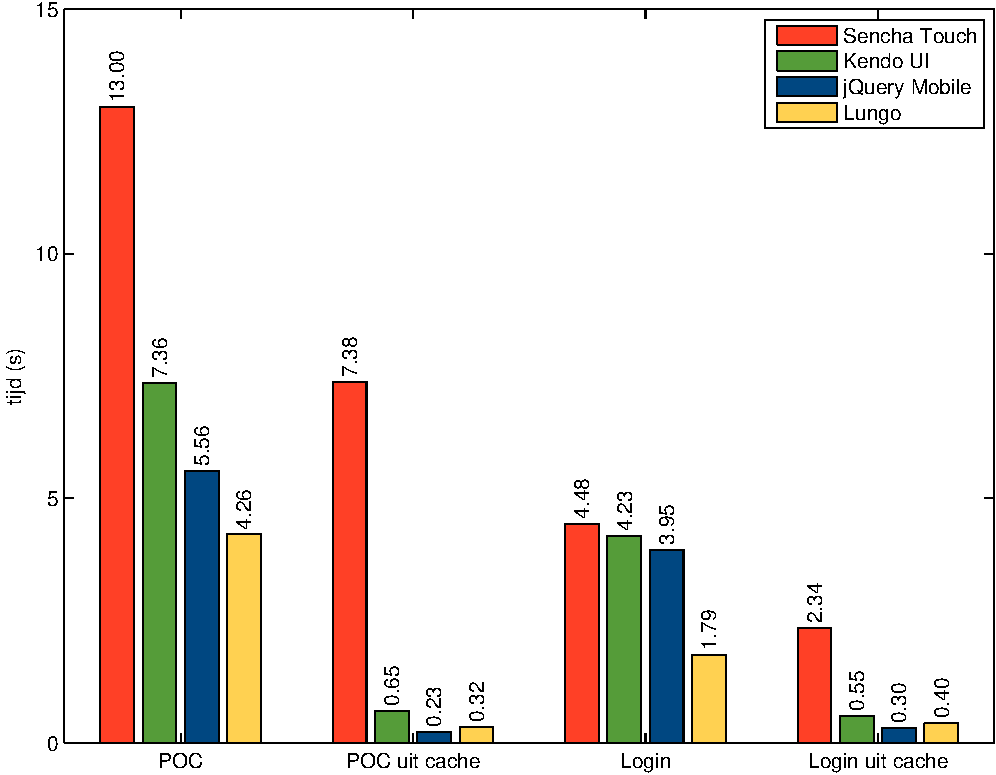
\includegraphics[width=\columnwidth]{../Masterproef/figuren/performance.pdf}
  \caption{Average download time for POC, POC from cache, login application, login application from cache for the four frameworks. Less is better.}
  \label{fig:evaluatie-performantie-gebruikerservaring}
\end{figure}

\lungo{} takes first place and only needs a third of the download time needed by \sta{}, the slowest of the four.
\jqma{} and \kendob{} take the second and third place respectively.
Because not everything was implemented in the POC of \lungo{}, one could argue that that is the reason of the first place of \lungo{}.
But when looking at the login application, \lungo{} still takes first place.
It is even more than half faster than \jqma{}, \kendob{} or \sta{}.
Those three frameworks have about the same average download time.
The reason that \kendob{} and \sta{} are respectively second last and last is because they enforce an architecture and therefore the libraries to download are bigger than those of \lungo{} and \jqma{}.

When viewing the cached versions of the POC and login application, \kendob{}, \jqma{} en \lungo{} have about the same average download time.
However \st{} has a much higher download time when using the cached version.
The first reason is that the first three frameworks are only using HTML5 Application Cache.
\sta{} also uses its own caching mechanism in addition to HTML5 Application Cache.
The second reason is that the application in the first three frameworks are compiled using Yeoman~\cite{Yeoman2013} and \st{} with Sencha Cmd~\cite{Sencha2012}.

%%%%%%%%%%%%%%%%%%

\paragraph{User experience}
Table \ref{tabel:evaluatie-performantie-gebruikerservaring} shows the total score for user experience.
\sta{} takes first place with the maximal score.
\jqma{} was voted six time the second best for user experience.
\kendob{} was better on the \htc{} and \lungo{} on the \ipadiii{}.
The generation of the 850 list items was impossible for \kendob{} on all the iOS devices.
The browser crashed an the device returned to the home screen.
%De reden alsook de grens waarom \kendo{} niet crasht op iOS-toestellen werd door tijdsbudget niet gecontroleerd.
%Een mogelijke denkpiste is dat \kendo{} een overhead genereerd die het maximale toegelaten geheugen voor het iOS-besturingssysteem overschrijdt.
In contrast, list generation did work on all Android devices.
%De score van \kendo{} is dus slechts voor vier apparaten.

\begin{table}
\centering
\pgfplotstabletypeset[
  begin table=\begin{tabular}{p{3cm} p{0.8cm} p{0.8cm} p{0.8cm} p{0.8cm} p{0.3cm}},
  end table=\end{tabular},
  skip coltypes=true,
  col sep=comma,
  string type,
  header=true,
  columns={Device,ST,Kendo,jQM,Lungo},
  columns/Device/.style={column name=\textbf{Device}, column type={l}},
  columns/ST/.style={column name=\textbf{\sta}, column type={l}},  
  columns/jQM/.style={column name=\textbf{\jqma}, column type={l}},    
  columns/Kendo/.style={column name=\textbf{\kendoa}, column type={l}},   
  columns/Lungo/.style={column name=\textbf{\lungoa}, column type={l}},   
  every head row/.style={
    before row=\toprule,
    after row=\midrule},
  every last row/.style={
  	before row=\midrule,
    after row=\bottomrule}
]{../Masterproef/tabellen/performantie-gebruikerservaring.csv}
\caption{User experience for \st{}~(\sta), \kendo{}~(\kendoa), \jqm{}~(\jqma) en \lungo{}~(\lungoa).}
\label{tabel:evaluatie-performantie-gebruikerservaring}
\end{table}

%%%%%%%%%%%%%%%%%%%%%%%%%%%%%%%%%%%%%%%%%%%%%%%%%%%%%%%%%%%%%%%%%%%%%%%%%%%%%%%%%%%%%%%

\subsection{Comparison overview} % ? blz
\label{sec:evaluation-overview}

Figure \ref{fig:spidergraph} shows the spidergraph with the scores for the five criteria for the four frameworks.

\jqma{} has the largest area ($1.87$) and can be seen as the winner.
One of the major factors that make \jqma{} successful is that it does not forces an architecture.
This decreases the learning curve in favor of productivity.
Also,  the extensive documentation and large community make \jqma{} more productive.
\lungo{} also forces no architecture but is extremely unpopular.
The absence of architecture also has two disadvantages.
First,  the framework provides less functionality but many plugins and HTML5-features act as substitutes.
Secondly,  the code that needs to be written is verbose and thereby error prone.

\kendob{} is second with an area of $1.32$.
The MVVM architecture makes \kendob{} more usable but less productive in comparison with \jqma{}.
However,  the MVVM arcitecture seems more intuitive than MVC.
The main drawback of \kendob{},  which can not be seen on the figure, is the high license kost.
The expectation that open-source frameworks are more popular is not reflected in the popularity scores.
\kendob{} also is the least performant.
The crashes on iOS devices caused a decrease in the user experience tests and hence a drop in performance.
The native look-and-feel and corresponding benefits are not been studied although it is an important factor for \kendob{} in particular.

\lungo{} has an area of ($0.88$) and claims the third place.
In tree out of five criteria,  \lungo{} is last.
For the other criteria,  \lungo{} is second.
Again, no architectur is imposed which can be seen in productivity and usability.
However,  the advantage in productivity is smaller and disadvantage is usability is larger in comparison with \jqma{}.
The lack of familiarity,  as can be seen with the popularity,  is an explanation of these differences.
A positive aspect is that \lungo{} achieved the best average download times.  
This is because \quo{},  the core library of \lungo{},  is optimised for mobile devices.
The user experience tests weakend the score for performance


\sta {} is has an area of ($0.73$) and is worst framework following these criteria.
The combination of the MVC architecture and the fact that it is \js-driven makes \sta{} both the least productive and least performant in comparison to the other frameworks.
Alle HTML code is generated by the framework and therefor the \js-files are very large.
As a result,  the average downloadtimes were remarkably large.
The user experience tests gave an opposite result because after the initial waiting time,  \sta{} had the fastest responstimes.
The tools provided by Sencha to support the developper are not able to close the gap in productivity.
The tools require a learning process on their own.
As a last remark,  \sta{} is depending on the WebKit engine.
Devices with a default browser that do not contain this engine,  like Windows Phone, are not investigated.

%TODO engelstalige labels maken
\begin{figure}
  \centering
  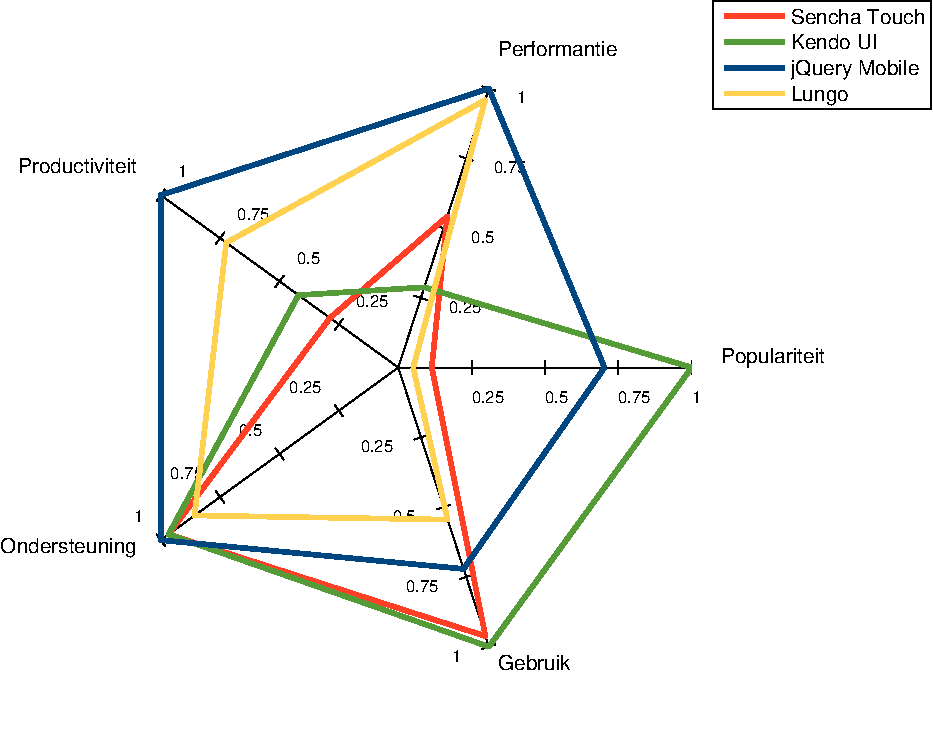
\includegraphics[width=\columnwidth]{../Masterproef/figuren/spidergraph-final.pdf}
  \caption{Overview with the five comparison criteria for \sta{},  \kendob{},  \jqma{} en \lungo{}.}
  \label{fig:spidergraph}
\end{figure}

%%%%%%%%%%%%%%%%%%%%%%%%%%%%%%%%%%%%%%%%%%%%%%%%%%%%%%%%%%%%%%%%%%%%%%%%%%%%%%%%%%%%%%%
%%%%%%%%%%%%%%%%%%%%%%%%%%%%%%%%%%%%%%%%%%%%%%%%%%%%%%%%%%%%%%%%%%%%%%%%%%%%%%%%%%%%%%%

\section{Future work} % 0,5 blz % Tim
\label{sec:future_work}
Firsty, one can look for deeper understanding why certain results are remarkable and why other things failed on particular devices.
An example of the former is why the average download time of the login from cache was higher than the POC from cache for both \jqma{} and \lungo{}.
An example for the latter is to search why the 850 list items of \kendob{} crashed on all iOS devices.
Furthermore research can be done to know the limit of list items when it starts crashing.

Secondly, one can add new frameworks to the comparison.
This will enlarge the comparison itself, but will also keep checking the method of comparing.
Furthermore, new versions of the compared framework will be published.
It may also be worth plotting the comparison over time.
This is because the ranking can change due to new features in framework or new plugins.

Thirdly, the five criteria are driven by the POC.
This POC can be further extended with extra features like a list that when it is pulled down, it automatically refreshes and fetches the new list items.
Similar to this action, one can also use other events than the tap event.
Examples of these are double tap, swipe, hold, and also events that require multiple fingers like a rotate event.
Furthermore the integration of HTML5 features likes GPS, push events, drag and drop, video and audio in frameworks can be researched.

Fourthly, new criteria can be added to the comparison.
It is off interest to incorporate extensibility which states how easy it is to extend an existing application.
A hypothesis is that framework that enforce an architecture will have better extensibility than framework who do not.
Furthermore this new criterion could change the current ranking of the four frameworks.
Another possible new criterion is to look at the final result of the application created by the framework.
Some framework make application that imitate the nativeness of the OS where they are viewed.
Other frameworks make application with an out-of-the-box modern lay-out.

Lastly, one can take a step back and research how web applications cope with battery usage.
This data can also be compared with native and hybrid applications.
This comparison can be more generalised and one can also compare between web, native and hybrid applications.

%%%%%%%%%%%%%%%%%%%%%%%%%%%%%%%%%%%%%%%%%%%%%%%%%%%%%%%%%%%%%%%%%%%%%%%%%%%%%%%%%%%%%%%
%%%%%%%%%%%%%%%%%%%%%%%%%%%%%%%%%%%%%%%%%%%%%%%%%%%%%%%%%%%%%%%%%%%%%%%%%%%%%%%%%%%%%%%

\section{Conclusion} % 0,5 blz % Sander
\label{sec:conclusion}

HTML5 is a newly,  not-standarised technology that targets mobile devices.
This technology provides an answer to the hetrogenity in devices, operatingsystems and browsers.
Many frameworks exist that are build upon HTML5 and facilitate the development of mobile web applications.

This paper described a comparative study between \sta{},  \kendob{},  \jqma{} and \lungo{}.
\sta{} is build with the MVC architecture and is \js-driven.
\kendob{} enforces the MVVM architecture and is both \js- as markupdriven.
\jqma{} and \lungo{} do not have an architecture and are both markupdriven.

Five criteria were chosen to execute the comparative study:  popularity,  productivity,  usage,  support and performance.
Each criterion was provided with a forumla to calculate a score for the criterion.
A POC was formalised and checked with the criteria in as many ways as possible.
The activity of the framework on social networks, determined the popularity.
The productivity was measured by timetracking the time to implementing a loginapplication.
The POC was subdivided in $13$ challenges and $38$ subchallenges to test the usability of the framework.
Next,  a subset of these challenges were tested on $8$ different devices to check the support.
Finally,  the load- and responsetime of the POC and loginapplication determined the performance criterion.
All the scores were plotted in a spidergraph.

The comparison shows that \jqm{} is the best framework.
Then, \kendo{},  \lungo{} and \st{} follow on respectively second, third and forth place.
\jqm{} has a high productivity and performance as major advantages because on the one hand it is well-documented and on the other hand it does not impose an architecture.
The latter,  however,  is a disadvantage when looking at the usability.
\kendo{} has the MVVM architecture as most important advantage.
However,  it scores below average because it crashes on iOS when loading long lists.
\lungo{} only achieved a maximumscore for perfomance because the framework is optimized for mobile usage.
\st{} is the least productive and performant in comparison with other frameworks.
By enforcing an architecture,  it scores almost as good as \kendo{} regarding usability.
All frameworks provide good support on the devices.

%%%%%%%%%%%%%%%%%%%%%%%%%%%%%%%%%%%%%%%%%%%%%%%%%%%%%%%%%%%%%%%%%%%%%%%%%%%%%%%%%%%%%%%
%%%%%%%%%%%%%%%%%%%%%%%%%%%%%%%%%%%%%%%%%%%%%%%%%%%%%%%%%%%%%%%%%%%%%%%%%%%%%%%%%%%%%%%

% % Define a new 'leo' style for the package that will use a smaller font.
% \makeatletter
% \def\url@leostyle{%
%   \@ifundefined{selectfont}{\def\UrlFont{\sf}}{\def\UrlFont{\small\ttfamily}}}
% \makeatother
% %% Now actually use the newly defined style.
% \urlstyle{leo}

%\bibliographystyle{named}
\bibliographystyle{abbrv}
\bibliography{../Referenties/alles-en}

\end{document}